\documentclass[logo,reportComp]{thesis}
\usepackage[cpp,pseudo]{mypackage}

\title{数据库系统实验}
\subtitle{Lab of MySQL}
\school{数据科学与计算机学院}
\author{陈鸿峥}
\classname{17大数据与人工智能}
\stunum{17341015}
\headercontext{数据库系统实验作业}

\lstset{language=sql}

\begin{document}

\maketitle
% https://www.db-book.com/db6/lab-dir/labexercises-dir/

具体代码请见下述四个程序文件,运行结果也都附在后文。
\begin{itemize}
\item \verb'BasicSQL-HW.sql':第二大题问题1到问题8
\item \verb'BasicSQL-HW2.sql':第二大题问题9到问题13
\item \verb'IntermediateSQL-HW.sql':第三大题问题1到问题5
\item \verb'IntermediateSQL-HW2.sql':第三大题问题6到问题10
\end{itemize}

\section{Accessing the Database}
需要先下载\verb'DDL-MySQL.sql'和\verb'smallRelationsInsertFile.sql'两个文件,然后用
\begin{lstlisting}
mysql -u root -p
\end{lstlisting}
进入MySQL界面,然后
\begin{lstlisting}
mysql> CREATE DATABASE school;
mysql> use school;
mysql> source DDL-MySQL.sql
mysql> source smallRelationsInsertFile.sql
\end{lstlisting}
即可进行实验。

\section{Basic SQL}
\begin{question}
\normalfont Find the names of all the instructors from Biology department
\end{question}
\begin{answer}\mbox{}\par
\begin{lstlisting}
select name
from instructor
where dept_name = 'Biology';
\end{lstlisting}
\end{answer}

\begin{question}
\normalfont 
Find the names of courses in Computer science department which have 3 credits
\end{question}
\begin{answer}\mbox{}\par
\begin{lstlisting}
select title
from course
where credits = 3;
\end{lstlisting}
\end{answer}

\begin{question}
\normalfont 
For the student with ID 12345 (or any other value), show all course\_id and title of all courses registered for by the student.
\end{question}
\begin{answer}\mbox{}\par
\begin{lstlisting}
select course_id, title
from takes natural join course
where ID = 12345;
\end{lstlisting}
\end{answer}

\begin{question}
\normalfont 
As above, but show the total number of credits for such courses (taken by that student). Don't display the tot\_creds value from the student table, you should use SQL aggregation on courses taken by the student.
\end{question}
\begin{answer}\mbox{}\par
\begin{lstlisting}
select sum(credits)
from takes natural join course
where ID = 12345;
\end{lstlisting}
\end{answer}

\begin{question}
\normalfont 
As above, but display the total credits for each of the students, along with the ID of the student; don't bother about the name of the student. (Don't bother about students who have not registered for any course, they can be omitted)
\end{question}
\begin{answer}\mbox{}\par
\begin{lstlisting}
select ID, sum(credits)
from takes natural join course
group by ID;
\end{lstlisting}
\end{answer}

\begin{question}
\normalfont 
Find the names of all students who have taken any Comp. Sci. course ever (there should be no duplicate names)
\end{question}
\begin{answer}\mbox{}\par
\begin{lstlisting}
select distinct S.name
from student as S, 
  (select * from takes natural join course) as C
where S.ID = C.ID and C.dept_name = 'Comp. Sci.';
\end{lstlisting}
\end{answer}

\begin{question}
\normalfont 
Display the IDs of all instructors who have never taught a couse. Note: (1) Oracle uses the keyword minus in place of except; (2) interpret "taught" as "taught or is scheduled to teach".
\end{question}
\begin{answer}注意MySQL没有\verb'except',故需要换种方式编写。
\begin{lstlisting}
-- (without except!)
select ID
from instructor
where ID not in
  (select ID
    from instructor natural join teaches);
\end{lstlisting}
\end{answer}

\begin{question}
\normalfont 
As above, but display the names of the instructors also, not just the IDs.
\end{question}
\begin{answer}\mbox{}\par
\begin{lstlisting}
select name, ID
from instructor
where ID not in
  (select ID
    from instructor natural join teaches);
\end{lstlisting}
\end{answer}

\begin{figure}[H]
\centering
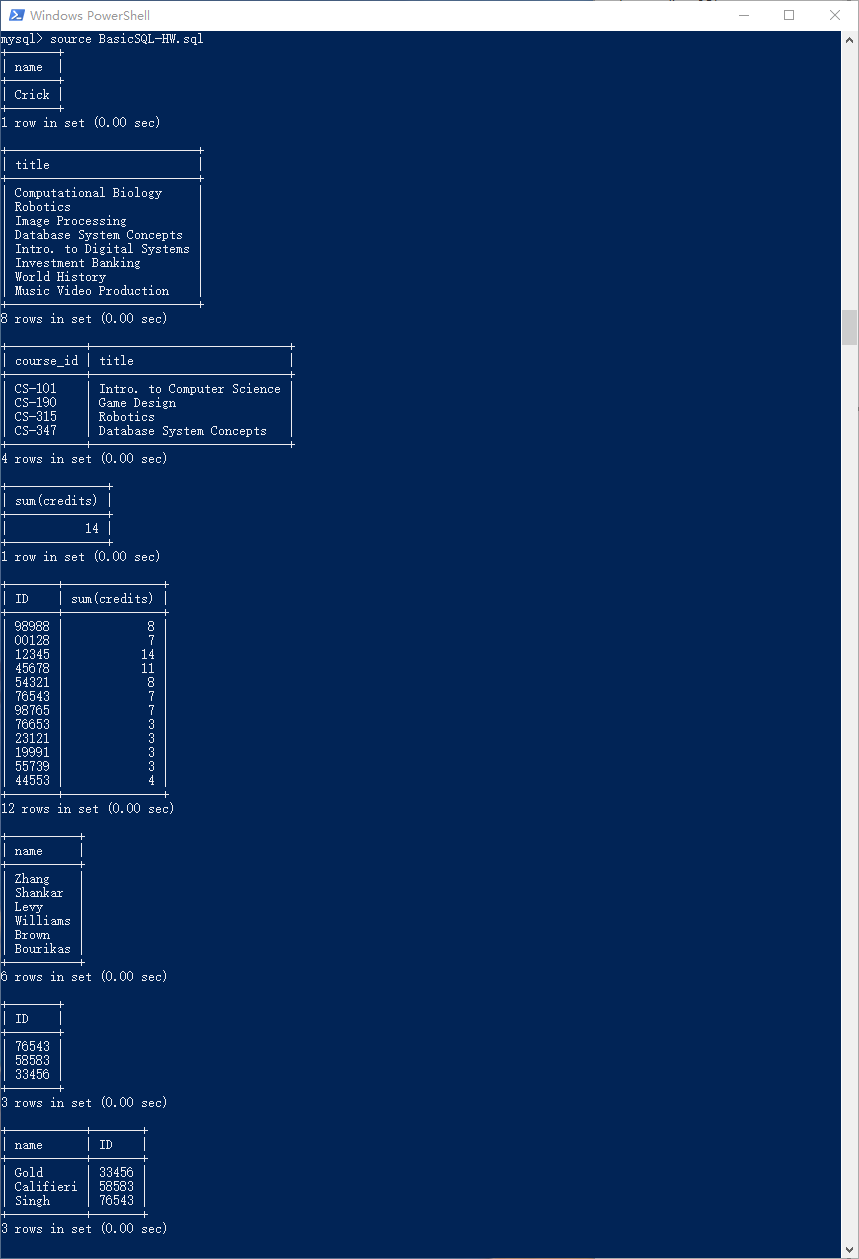
\includegraphics[width=\linewidth]{fig/Q1-8.png}
\caption{问题1到8结果}
\end{figure}

\begin{question}
\normalfont 
You need to create a movie database. Create three tables, one for actors(AID, name), one for movies(MID, title) and one for actor\_role(MID, AID, rolename). Use appropriate data types for each of the attributes, and add appropriate primary/foreign key constraints.
\end{question}
\begin{answer}\mbox{}\par
\begin{lstlisting}
create table actors
  (AID    varchar(20),
   name   varchar(50),
   primary key (AID));

create table movies
  (MID    varchar(20),
   title  varchar(50),
   primary key (MID));

create table actor_role
  (MID    varchar(20),
   AID    varchar(20),
   rolename varchar(30),
   primary key (MID,AID,rolename),
   foreign key (MID) references movies(MID),
   foreign key (AID) references actors(AID));
\end{lstlisting}
\end{answer}

\begin{question}
\normalfont 
Insert data to the above tables (approx 3 to 6 rows in each table), including data for actor "Charlie Chaplin", and for yourself (using your roll number as ID).
\end{question}
\begin{answer}\mbox{}\par
\begin{lstlisting}
delete from actor_role;
delete from actors;
delete from movies;
insert into actors values ('01','Charlie Chaplin');
insert into movies values ('M1','Modern Times');
insert into actor_role values ('M1','01','Worker');
insert into movies values ('M2','The Great Dictator');
insert into actor_role values ('M2','01','Adenoid');
insert into actor_role values ('M2','01','Barber');
insert into movies values ('M3','City Lights');
insert into actor_role values ('M3','01','Tramp');
insert into actors values ('02','Leslie Cheung');
insert into movies values ('M4','Farewell My Concubine');
insert into actor_role values ('M4','02','Dieyi Cheng');
insert into actors values ('03','Tom Hanks');
insert into movies values ('M5','Forrest Gump');
insert into actor_role values ('M5','03','Gump');
insert into actors values ('04','No-movie Actor');
\end{lstlisting}
\end{answer}

\begin{question}
\normalfont 
Write a query to list all movies in which actor "Charlie Chaplin" has acted, along with the number of roles he had in that movie.
\end{question}
\begin{answer}\mbox{}\par
\begin{lstlisting}
select name, title, count(rolename)
from actor_role natural join movies natural join actors
where name = 'Charlie Chaplin'
group by MID;
\end{lstlisting}
\end{answer}

\begin{question}
\normalfont 
Write a query to list all actors who have not acted in any movie
\end{question}
\begin{answer}这里创建视图(view)是为了下一问比较好做,如果单独只做这一问则可以不创建。
\begin{lstlisting}
create view no_movie_actor as
select name
from actors
where name not in (select distinct name
          from actor_role natural join actors);
select * from no_movie_actor;
\end{lstlisting}
\end{answer}

\begin{question}
\normalfont 
List names of actors, along with titles of movies they have acted in. If they have not acted in any movie, show the movie title as null. (Do not use SQL outerjoin syntax here, write it from scratch.)
\end{question}
\begin{answer}这里不用outerjoin,只好先创建null的行,再进行整合。
\begin{lstlisting}
select *
from ((select name, title
    from actors, movies, actor_role
    where actors.AID = actor_role.AID and movies.MID = actor_role.MID)
  union
  (select name as name, null as title
    from no_movie_actor))
  as result;
\end{lstlisting}
\end{answer}

\begin{figure}[H]
\centering
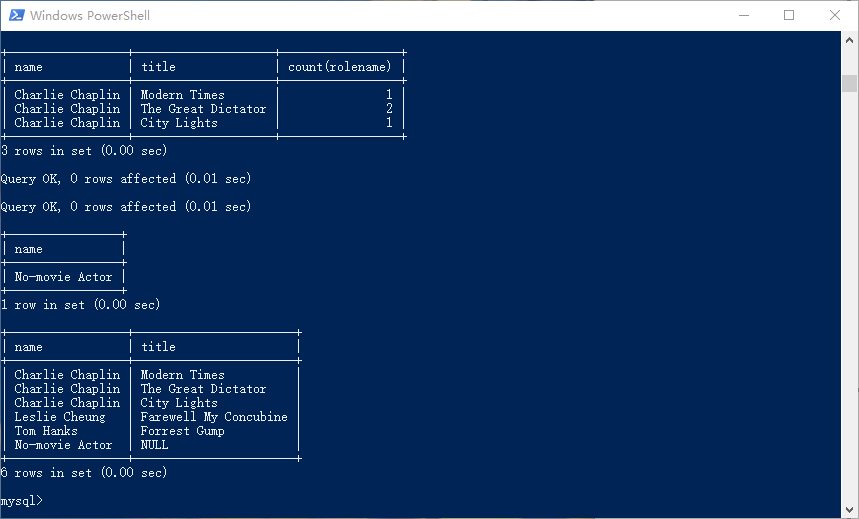
\includegraphics[width=\linewidth]{fig/Q9-13.png}
\caption{问题11到13结果,问题9、问题10的结果由于全是Query OK,故这里忽略}
\end{figure}

\setcounter{question}{0}
\section{Intermediate SQL}
Using the university schema that you have write the following queries. In some cases you need to insert extra data to show the effect of a particular feature -- this is indicated with the question. You should then show not only the query, but also the insert statements to add the required extra data.

\begin{question}
\normalfont 
Find the maximum and minimum enrollment across all sections, considering only sections that had some enrollment, don't worry about those that had no students taking that section
\end{question}
\begin{answer}\mbox{}\par
\begin{lstlisting}
select max(enrollment), min(enrollment)
from (select sec_id, semester, year, count(distinct id) as enrollment
  from takes
  group by sec_id, semester, year) as T;
\end{lstlisting}
\end{answer}

\begin{question}
\normalfont 
Find all sections that had the maximum enrollment (along with the enrollment), using a subquery.
\end{question}
\begin{answer}这里复用了上一问的语句。
\begin{lstlisting}
with T(sec_id, semester, year, enrollment) as
  (select sec_id, semester, year, count(distinct id)
    from takes
    group by sec_id, semester, year)
select T.sec_id, T.semester, T.year, T.enrollment
from T, (select max(enrollment) as maxE, min(enrollment)
  from T) as res
where T.enrollment = res.maxE;
\end{lstlisting}
\end{answer}

\begin{question}
\normalfont 
As in in Q1, but now also include sections with no students taking them; the enrollment for such sections should be treated as 0. Do this in two different ways (and create require data for testing)
\begin{itemize}
\item [(a)] Using a scalar subquery
\item [(b)] Using aggregation on a left outer join (use the SQL natural left outer join syntax)
\end{itemize}
\end{question}
\begin{answer}注意在添加元组时都需要保持约束的可满足性。
\begin{lstlisting}
-- Test data (need to preserve the constraints)
delete from course
  where course_id = 'CS-001';
delete from section
  where sec_id = '1' and semester = 'Fall' and year = '2010';
insert into course(course_id)
  values ('CS-001');
insert into section(course_id, sec_id, semester, year)
  values ('CS-001','1','Fall','2010');
-- Q3.1
select distinct sec_id, semester, year,
  (select count(distinct id)
    from takes
    where (takes.sec_id, takes.semester, takes.year) = (section.sec_id, section.semester, section.year)) as cnt
from section;
-- Q3.2
select distinct sec_id, semester, year, ifnull(cnt,0)
from section left outer join
  (select sec_id, semester, year, count(distinct id) as cnt
  from takes
  group by sec_id, semester, year) as T
using (sec_id, semester, year);
\end{lstlisting}
\end{answer}

\begin{question}
\normalfont 
Find all courses whose identifier starts with the string "CS-1"
\end{question}
\begin{answer}\mbox{}\par
\begin{lstlisting}
select course_id, title
from section natural join course
where course_id like 'CS-1%';
\end{lstlisting}
\end{answer}

\begin{question}
\normalfont 
Find instructors who have taught all the above courses
\begin{itemize}
\item [(a)] Using the "not exists ... except ..." structure
\item [(b)] Using matching of counts which we covered in class (don't forget the distinct clause!).
\end{itemize}
\end{question}
\begin{answer}由于MySQL没有\verb'except'语法,故这里同样需要采用其他方法代替(not in)。
\begin{lstlisting}
-- Q5.1
select distinct ID, name
from (select * from teaches natural join instructor) as T
where not exists (select cs_course.course_id
        from (select course_id
            from course
            where course_id like 'CS-1%') as cs_course
        where cs_course.course_id not in
          (select course_id
            from (select * from teaches natural join instructor) as U
            where U.name = T.name));

-- Q5.2
with U(course_id) as -- all course_id like 'CS-1%'
  (select distinct course_id
    from teaches natural join instructor
    where course_id like 'CS-1%')
select distinct ID, name
from (select * from teaches natural join instructor) as T
where ((select count(distinct course_id)
    from teaches natural join instructor
    where name = T.name and course_id like 'CS-1%')
  = (select count(course_id) from U));
\end{lstlisting}
\end{answer}

\begin{figure}[H]
\centering
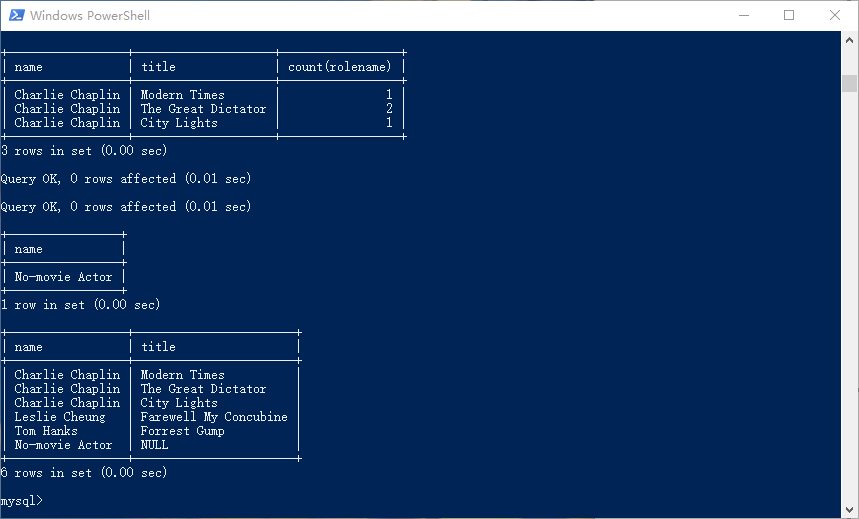
\includegraphics[width=\linewidth]{fig/Q9-13.png}
\caption{问题1到5结果}
\end{figure}

\begin{question}
\normalfont 
Insert each instructor as a student, with tot\_creds = 0, in the same department
\end{question}
\begin{answer}\mbox{}\par
\begin{lstlisting}
insert into student
  select ID, name, dept_name, '0'
  from instructor;
\end{lstlisting}
由于学生和老师的ID冲突,直接运行会报以下错误
\begin{lstlisting}
ERROR 1062 (23000): Duplicate entry '76543' for key 'PRIMARY'
\end{lstlisting}
\end{answer}

\begin{question}
\normalfont 
Now delete all the newly added "students" above (note: already existing students who happened to have tot\_creds = 0 should not get deleted)
\end{question}
\begin{answer}\mbox{}\par
\begin{lstlisting}
delete from student
  where (ID, name, dept_name) in
    (select ID, name, dept_name
      from instructor);
\end{lstlisting}
由于上一问没有插入成功,因此这一问也不会产生删除,运行会得到
\begin{lstlisting}
Query OK, 0 rows affected (0.00 sec)
\end{lstlisting}
\end{answer}

\begin{question}
\normalfont 
Some of you may have noticed that the tot\_creds value for students did not match the credits from courses they have taken. Write and execute query to update tot\_creds based on the credits passed, to bring the database back to consistency. (This query is provided in the book/slides.)
\end{question}
\begin{answer}\mbox{}\par
\begin{lstlisting}
update student as S
set tot_cred = (
  select sum(credits)
  from takes natural join course
  where S.ID = takes.ID and takes.grade is not null);
\end{lstlisting}
\begin{figure}[H]
\centering
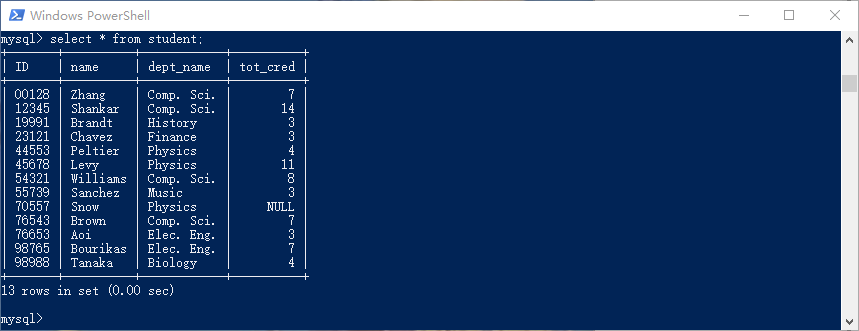
\includegraphics[width=\linewidth]{fig/Q8.png}
\caption{问题8结果}
\end{figure}
\end{answer}

\begin{question}
\normalfont 
Update the salary of each instructor to 10000 times the number of course sections they have taught.
\end{question}
\begin{answer}\mbox{}\par
\begin{lstlisting}
update instructor as I
set salary = 10000 * (
  select count(distinct sec_id, semester, year)
  from teaches as T
  where I.ID = T.ID);
\end{lstlisting}
由于部分老师上了3节课,薪酬变为30000美元,但与数据库的约束条件冲突,故直接运行会产生以下错误。
\begin{lstlisting}
ERROR 3819 (HY000): Check constraint 'instructor_chk_1' is violated.
\end{lstlisting}
\end{answer}

\begin{question}
\normalfont 
Create your own query: define what you want to do in English, then write the query in SQL. Make it as difficult as you wish, the harder the better.
\end{question}
\begin{answer}
这里我设计的问题是,统计由CS系教授开设的且被学生注册的课程总数。
这里既采用了子查询,又使用了聚集函数等。
\begin{lstlisting}
-- Number of courses taught by instuctors of CS department registered by the students
select count(cs_course.course_id)
from ((select distinct course_id
    from instructor natural join teaches
    where dept_name = 'Comp. Sci.') as cs_course
  inner join
  (select distinct course_id from takes) as all_course
  on cs_course.course_id = all_course.course_id);
\end{lstlisting}
\begin{figure}[H]
\centering
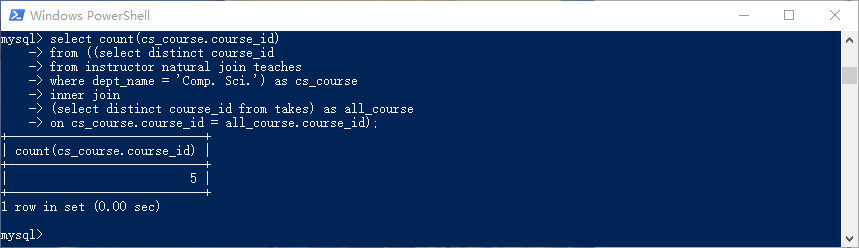
\includegraphics[width=\linewidth]{fig/Q10.png}
\caption{问题10结果}
\end{figure}
\end{answer}


\end{document}